\documentclass[twocolumn]{aastex62}
%\documentclass[defaultstyle,11pt]{thesis}
%\documentclass[]{report}
%\documentclass[]{article}
%\usepackage{aastex_hack}
%\usepackage{deluxetable}
%\documentclass[preprint]{aastex}
%\documentclass{aa}

\newcommand{\titlerunning}[1]{\shorttitle{#1}}
\newcommand{\authorrunning}[1]{\shortauthors{#1}}

\newcommand*\inst[1]{\unskip\hbox{\@textsuperscript{\normalfont$#1$}}}

%\newcount\aa@nbinstitutes
%
%\newcounter{aa@institutecnt}

\newcommand*\institute[1]{
  \begingroup
    \let\and\relax
    \renewcommand*\inst[1]{}%
    \renewcommand*\thanks[1]{}%
    \renewcommand*\email[1]{}%
    %\let\@@protect\protect
    %\let\protect\@unexpandable@protect
    %\global\aa@nbinstitutes \z@
    %\expandafter\aa@cntinstitutes\aa@institute\and\aa@nil\and
    %\restore@protect
  \endgroup
  \newcommand{\institutions}{#1}
}%

\let\oldarcsec\arcsec
\renewcommand\arcsec{\oldarcsec\xspace}%

%\renewcommand{\abstract}[1]{
%\begin{abstract}
%    #1
%\end{abstract}
%}

%\renewcommand\ion[2]{#1$\;${%
%\ifx\@currsize\normalsize\small \else
%\ifx\@currsize\small\footnotesize \else
%\ifx\@currsize\footnotesize\scriptsize \else
%\ifx\@currsize\scriptsize\tiny \else
%\ifx\@currsize\large\normalsize \else
%\ifx\@currsize\Large\large
%\fi\fi\fi\fi\fi\fi
%\rmfamily\@Roman{#2}}\relax}% 
%
%\renewcommand{ion}[2]{#1}{#2}

\renewcommand{\ion}[2]{\textup{#1\,\textsc{\lowercase{#2}}}}

%\newcommand{\uchii}{\ensuremath{\mathrm{\ion{UCH}{2}}}\xspace}
%\newcommand{\UCHII}{\ensuremath{\mathrm{\ion{UCH}{2}}}\xspace}
%\newcommand{\hchii}{\ensuremath{\mathrm{\ion{HCH}{2}}}\xspace}
%\newcommand{\HCHII}{\ensuremath{\mathrm{\ion{HCH}{2}}}\xspace}
%\newcommand{\hii}  {\ensuremath{\mathrm{\ion{H}{2}}}\xspace}

%\input{aamacros.tex}

\pdfminorversion=4


%%%%%%%%%%%%%%%%%%%%%%%%%%%%%%%%%%%%%%%%%%%%%%%%%%%%%%%%%%%%%%%%
%%%%%%%%%%%  see documentation for information about  %%%%%%%%%%
%%%%%%%%%%%  the options (11pt, defaultstyle, etc.)   %%%%%%%%%%
%%%%%%%  http://www.colorado.edu/its/docs/latex/thesis/  %%%%%%%
%%%%%%%%%%%%%%%%%%%%%%%%%%%%%%%%%%%%%%%%%%%%%%%%%%%%%%%%%%%%%%%%
%		\documentclass[typewriterstyle]{thesis}
% 		\documentclass[modernstyle]{thesis}
% 		\documentclass[modernstyle,11pt]{thesis}
%	 	\documentclass[modernstyle,12pt]{thesis}

%%%%%%%%%%%%%%%%%%%%%%%%%%%%%%%%%%%%%%%%%%%%%%%%%%%%%%%%%%%%%%%%
%%%%%%%%%%%    load any packages which are needed    %%%%%%%%%%%
%%%%%%%%%%%%%%%%%%%%%%%%%%%%%%%%%%%%%%%%%%%%%%%%%%%%%%%%%%%%%%%%
\usepackage{latexsym}		% to get LASY symbols
\usepackage{graphicx}		% to insert PostScript figures
%\usepackage{deluxetable}
\usepackage{rotating}		% for sideways tables/figures
\usepackage{natbib}  % Requires natbib.sty, available from http://ads.harvard.edu/pubs/bibtex/astronat/
\usepackage{savesym}
%\usepackage{pdflscape}
\usepackage{amssymb}
\usepackage{amsmath}
\usepackage{morefloats}
%\savesymbol{singlespace}
\savesymbol{doublespace}
%\usepackage{wrapfig}
%\usepackage{setspace}
\usepackage{xspace}
\usepackage{color}
%\usepackage{multicol}
\usepackage{mdframed}
\usepackage{url}
\usepackage{subfigure}
%\usepackage{emulateapj}
%\usepackage{lscape}
\usepackage{grffile}
\usepackage{import}
\usepackage[utf8]{inputenc}
%\usepackage{longtable}
\usepackage{booktabs}
%\usepackage[yyyymmdd,hhmmss]{datetime}
\usepackage{fancyhdr}
%\usepackage[colorlinks=true,citecolor=blue,linkcolor=cyan]{hyperref}

\usepackage[hang,flushmargin]{footmisc}
\usepackage{ifpdf}


%\usepackage{standalone}
%\standalonetrue






\newcommand{\paa}{Pa\ensuremath{\alpha}}
\newcommand{\brg}{Br\ensuremath{\gamma}}
\newcommand{\msun}{\ensuremath{M_{\odot}}\xspace}			%  Msun
\newcommand{\mdot}{\ensuremath{\dot{M}}\xspace}
\newcommand{\lsun}{\ensuremath{L_{\odot}}\xspace}			%  Lsun
\newcommand{\rsun}{\ensuremath{R_{\odot}}\xspace}			%  Rsun
\newcommand{\lbol}{\ensuremath{L_{\mathrm{bol}}\xspace}}	%  Lbol
\newcommand{\ks}{K\ensuremath{_{\mathrm{s}}}}		%  Ks
\newcommand{\hh}{\ensuremath{\textrm{H}_{2}}\xspace}			%  H2
\newcommand{\dens}{\ensuremath{n(\hh) [\percc]}\xspace}
\newcommand{\formaldehyde}{\ensuremath{\textrm{H}_2\textrm{CO}}\xspace}
\newcommand{\formamide}{\ensuremath{\textrm{NH}_2\textrm{CHO}}\xspace}
\newcommand{\formaldehydeIso}{\ensuremath{\textrm{H}_2~^{13}\textrm{CO}}\xspace}
\newcommand{\methanol}{\ensuremath{\textrm{CH}_3\textrm{OH}}\xspace}
\newcommand{\ortho}{\ensuremath{\textrm{o-H}_2\textrm{CO}}\xspace}
\newcommand{\para}{\ensuremath{\textrm{p-H}_2\textrm{CO}}\xspace}
\newcommand{\oneone}{\ensuremath{1_{1,0}-1_{1,1}}\xspace}
\newcommand{\twotwo}{\ensuremath{2_{1,1}-2_{1,2}}\xspace}
\newcommand{\threethree}{\ensuremath{3_{1,2}-3_{1,3}}\xspace}
\newcommand{\threeohthree}{\ensuremath{3_{0,3}-2_{0,2}}\xspace}
\newcommand{\threetwotwo}{\ensuremath{3_{2,2}-2_{2,1}}\xspace}
\newcommand{\threetwoone}{\ensuremath{3_{2,1}-2_{2,0}}\xspace}
\newcommand{\fourtwotwo}{\ensuremath{4_{2,2}-3_{1,2}}\xspace} % CH3OH 218.4 GHz
\newcommand{\methylcyanide}{\ensuremath{\textrm{CH}_{3}\textrm{CN}}\xspace}
\newcommand{\ketene}{\ensuremath{\textrm{H}_{2}\textrm{CCO}}\xspace}
\newcommand{\ethylcyanide}{\ensuremath{\textrm{CH}_3\textrm{CH}_2\textrm{CN}}\xspace}
\newcommand{\cyanoacetylene}{\ensuremath{\textrm{HC}_{3}\textrm{N}}\xspace}
\newcommand{\methylformate}{\ensuremath{\textrm{CH}_{3}\textrm{OCHO}}\xspace}
\newcommand{\dimethylether}{\ensuremath{\textrm{CH}_{3}\textrm{OCH}_{3}}\xspace}
\newcommand{\gaucheethanol}{\ensuremath{\textrm{g-CH}_3\textrm{CH}_2\textrm{OH}}\xspace}
\newcommand{\acetone}{\ensuremath{\left[\textrm{CH}_{3}\right]_2\textrm{CO}}\xspace}
\newcommand{\methyleneamidogen}{\ensuremath{\textrm{H}_{2}\textrm{CN}}\xspace}
\newcommand{\Rone}{\ensuremath{\para~S_{\nu}(\threetwoone) / S_{\nu}(\threeohthree)}\xspace}
\newcommand{\Rtwo}{\ensuremath{\para~S_{\nu}(\threetwotwo) / S_{\nu}(\threetwoone)}\xspace}
\newcommand{\JKaKc}{\ensuremath{J_{K_a K_c}}}
\newcommand{\water}{H$_{2}$O\xspace}		%  H2O
\newcommand{\feii}{\ion{Fe}{ii}\xspace}		%  FeII

\newcommand{\uchii}{\ion{UCH}{ii}\xspace}
\newcommand{\UCHII}{\ion{UCH}{ii}\xspace}
\newcommand{\hchii}{\ion{HCH}{ii}\xspace}
\newcommand{\HCHII}{\ion{HCH}{ii}\xspace}
\newcommand{\hii}{\ion{H}{ii}\xspace}

\newcommand{\hi}{H~{\sc i}\xspace}
\newcommand{\Hii}{\hii}
\newcommand{\HII}{\hii}
\newcommand{\Xform}{\ensuremath{X_{\formaldehyde}}}
\newcommand{\kms}{\textrm{km~s}\ensuremath{^{-1}}\xspace}	%  km s-1
\newcommand{\nsample}{456\xspace}
\newcommand{\CFR}{5\xspace} % nMPC / 0.25 / 2 (6 for W51 once, 8 for W51 twice) REFEDIT: With f_observed=0.3, becomes 3/2./0.3 = 5
\newcommand{\permyr}{\ensuremath{\mathrm{Myr}^{-1}}\xspace}
\newcommand{\pers}{\ensuremath{\mathrm{s}^{-1}}\xspace}
\newcommand{\perspc}{\ensuremath{\mathrm{pc}^{-2}}\xspace}
\newcommand{\tsuplim}{0.5\xspace} % upper limit on starless timescale
\newcommand{\ncandidates}{18\xspace}
\newcommand{\mindist}{8.7\xspace}
\newcommand{\rcluster}{2.5\xspace}
\newcommand{\ncomplete}{13\xspace}
\newcommand{\middistcut}{13.0\xspace}
\newcommand{\nMPC}{3\xspace} % only count W51 once.  W51, W49, G010
\newcommand{\obsfrac}{30}
\newcommand{\nMPCtot}{10\xspace} % = nmpc / obsfrac
\newcommand{\nMPCtoterr}{6\xspace} % = sqrt(nmpc) / obsfrac
\newcommand{\plaw}{2.1\xspace}
\newcommand{\plawerr}{0.3\xspace}
\newcommand{\mmin}{\ensuremath{10^4~\msun}\xspace}
%\newcommand{\perkmspc}{\textrm{per~km~s}\ensuremath{^{-1}}\textrm{pc}\ensuremath{^{-1}}\xspace}	%  km s-1 pc-1
\newcommand{\kmspc}{\textrm{km~s}\ensuremath{^{-1}}\textrm{pc}\ensuremath{^{-1}}\xspace}	%  km s-1 pc-1
\newcommand{\sqcm}{cm$^{2}$\xspace}		%  cm^2
\newcommand{\percc}{\ensuremath{\textrm{cm}^{-3}}\xspace}
\newcommand{\perpc}{\ensuremath{\textrm{pc}^{-1}}\xspace}
\newcommand{\persc}{\ensuremath{\textrm{cm}^{-2}}\xspace}
\newcommand{\persr}{\ensuremath{\textrm{sr}^{-1}}\xspace}
\newcommand{\peryr}{\ensuremath{\textrm{yr}^{-1}}\xspace}
\newcommand{\perkmspc}{\textrm{km~s}\ensuremath{^{-1}}\textrm{pc}\ensuremath{^{-1}}\xspace}	%  km s-1 pc-1
\newcommand{\perkms}{\textrm{per~km~s}\ensuremath{^{-1}}\xspace}	%  km s-1 
\newcommand{\um}{\ensuremath{\mu \textrm{m}}\xspace}    % micron
\newcommand{\microjy}{\ensuremath{\mu\textrm{Jy}}\xspace}    % micron
\newcommand{\microJy}{\ensuremath{\mu\textrm{Jy}}\xspace}    % micron
\newcommand{\mum}{\um}
\newcommand{\htwo}{\ensuremath{\textrm{H}_2}}
\newcommand{\Htwo}{\ensuremath{\textrm{H}_2}}
\newcommand{\HtwoO}{\ensuremath{\textrm{H}_2\textrm{O}}}
\newcommand{\htwoo}{\ensuremath{\textrm{H}_2\textrm{O}}}
\newcommand{\ha}{\ensuremath{\textrm{H}\alpha}}
\newcommand{\hb}{\ensuremath{\textrm{H}\beta}}
\newcommand{\so}{SO~\ensuremath{5_6-4_5}\xspace}
\newcommand{\SO}{SO~\ensuremath{1_2-1_1}\xspace}
\newcommand{\ammonia}{NH\ensuremath{_3}\xspace}
\newcommand{\twelveco}{\ensuremath{^{12}\textrm{CO}}\xspace}
\newcommand{\thirteenco}{\ensuremath{^{13}\textrm{CO}}\xspace}
\newcommand{\ceighteeno}{\ensuremath{\textrm{C}^{18}\textrm{O}}\xspace}
\def\ee#1{\ensuremath{\times10^{#1}}}
\newcommand{\degrees}{\ensuremath{^{\circ}}}
% can't have \degree because I'm getting a degree...
\newcommand{\lowirac}{800}
\newcommand{\highirac}{8000}
\newcommand{\lowmips}{600}
\newcommand{\highmips}{5000}
\newcommand{\perbeam}{\ensuremath{\textrm{beam}^{-1}}\xspace}
\newcommand{\ds}{\ensuremath{\textrm{d}s}}
\newcommand{\dnu}{\ensuremath{\textrm{d}\nu}}
\newcommand{\dv}{\ensuremath{\textrm{d}v}}
\def\secref#1{Section \ref{#1}}
\def\eqref#1{Equation \ref{#1}}
\def\facility#1{#1}
%\newcommand{\arcmin}{'}

\newcommand{\necluster}{Sh~2-233IR~NE}
\newcommand{\swcluster}{Sh~2-233IR~SW}
\newcommand{\region}{IRAS 05358}

\newcommand{\nwfive}{40}
\newcommand{\nouter}{15}

\newcommand{\vone}{{\rm v}1.0\xspace}
\newcommand{\vtwo}{{\rm v}2.0\xspace}
\newcommand\mjysr{\ensuremath{{\rm MJy~sr}^{-1}}}
\newcommand\jybm{\ensuremath{{\rm Jy~bm}^{-1}}}
\newcommand\nbolocat{8552\xspace}
\newcommand\nbolocatnew{548\xspace}
\newcommand\nbolocatnonew{8004\xspace} % = nbolocat-nbolocatnew
%\renewcommand\arcdeg{\mbox{$^\circ$}\xspace} 
%\renewcommand\arcmin{\mbox{$^\prime$}\xspace} 
%\renewcommand\arcsec{\mbox{$^{\prime\prime}$}\xspace} 

\newcommand{\todo}[1]{\textcolor{red}{#1}}
\newcommand{\okinfinal}[1]{{#1}}
%% only needed if not aastex
%\newcommand{\keywords}[1]{}
%\newcommand{\email}[1]{}
%\newcommand{\affil}[1]{}


%aastex hack
%\newcommand\arcdeg{\mbox{$^\circ$}}%
%\newcommand\arcmin{\mbox{$^\prime$}\xspace}%
%\newcommand\arcsec{\mbox{$^{\prime\prime}$}\xspace}%

%\newcommand\epsscale[1]{\gdef\eps@scaling{#1}}
%
%\newcommand\plotone[1]{%
% \typeout{Plotone included the file #1}
% \centering
% \leavevmode
% \includegraphics[width={\eps@scaling\columnwidth}]{#1}%
%}%
%\newcommand\plottwo[2]{{%
% \typeout{Plottwo included the files #1 #2}
% \centering
% \leavevmode
% \columnwidth=.45\columnwidth
% \includegraphics[width={\eps@scaling\columnwidth}]{#1}%
% \hfil
% \includegraphics[width={\eps@scaling\columnwidth}]{#2}%
%}}%


%\newcommand\farcm{\mbox{$.\mkern-4mu^\prime$}}%
%\let\farcm\farcm
%\newcommand\farcs{\mbox{$.\!\!^{\prime\prime}$}}%
%\let\farcs\farcs
%\newcommand\fp{\mbox{$.\!\!^{\scriptscriptstyle\mathrm p}$}}%
%\newcommand\micron{\mbox{$\mu$m}}%
%\def\farcm{%
% \mbox{.\kern -0.7ex\raisebox{.9ex}{\scriptsize$\prime$}}%
%}%
%\def\farcs{%
% \mbox{%
%  \kern  0.13ex.%
%  \kern -0.95ex\raisebox{.9ex}{\scriptsize$\prime\prime$}%
%  \kern -0.1ex%
% }%
%}%

\def\Figure#1#2#3#4#5{
\begin{figure*}[!htp]
\includegraphics[scale=#4,width=#5]{#1}
\caption{#2}
\label{#3}
\end{figure*}
}

\def\FigureOneCol#1#2#3#4#5{
\begin{figure}[!htp]
\includegraphics[scale=#4,width=#5]{#1}
\caption{#2}
\label{#3}
\end{figure}
}


\def\WrapFigure#1#2#3#4#5#6{
\begin{wrapfigure}{#6}{0.5\textwidth}
\includegraphics[scale=#4,width=#5]{#1}
\caption{#2}
\label{#3}
\end{wrapfigure}
}

% % #1 - filename
% % #2 - caption
% % #3 - label
% % #4 - epsscale
% % #5 - R or L?
% \def\WrapFigure#1#2#3#4#5#6{
% \begin{wrapfigure}[#6]{#5}{0.45\textwidth}
% %  \centercaption
% %  \vspace{-14pt}
%   \epsscale{#4}
%   \includegraphics[scale=#4]{#1}
%   \caption{#2}
%   \label{#3}
% \end{wrapfigure}
% }

\def\RotFigure#1#2#3#4#5{
\begin{sidewaysfigure*}[!htp]
\includegraphics[scale=#4,width=#5]{#1}
\caption{#2}
\label{#3}
\end{sidewaysfigure*}
}

\def\FigureSVG#1#2#3#4{
\begin{figure*}[!htp]
    \def\svgwidth{#4}
    \input{#1}
    \caption{#2}
    \label{#3}
\end{figure*}
}

% originally intended to be included in a two-column paper
% this is in includegraphics: ,width=3in
% but, not for thesis
\def\OneColFigure#1#2#3#4#5{
\begin{figure}[!htpb]
\epsscale{#4}
\includegraphics[scale=#4,angle=#5]{#1}
\caption{#2}
\label{#3}
\end{figure}
}

\def\SubFigure#1#2#3#4#5{
\begin{figure*}[!htp]
\addtocounter{figure}{-1}
\epsscale{#4}
\includegraphics[angle=#5]{#1}
\caption{#2}
\label{#3}
\end{figure*}
}


\def\FigureTwo#1#2#3#4#5#6{
\begin{figure*}[!htp]
\subfigure[]{ \includegraphics[scale=#5,width=#6]{#1} }
\subfigure[]{ \includegraphics[scale=#5,width=#6]{#2} }
\caption{#3}
\label{#4}
\end{figure*}
}

\def\FigureTwoAA#1#2#3#4#5#6{
\begin{figure*}[!htp]
\subfigure[]{ \includegraphics[scale=#5,width=#6]{#1} }
\subfigure[]{ \includegraphics[scale=#5,width=#6]{#2} }
\caption{#3}
\label{#4}
\end{figure*}
}

\newenvironment{rotatepage}
{}{}


\def\RotFigureTwoAA#1#2#3#4#5#6{
\begin{rotatepage}
\begin{sidewaysfigure*}[!htp]
\subfigure[]{ \includegraphics[scale=#5,width=#6]{#1} }
\\
\subfigure[]{ \includegraphics[scale=#5,width=#6]{#2} }
\caption{#3}
\label{#4}
\end{sidewaysfigure*}
\end{rotatepage}
}

\def\RotFigureThree#1#2#3#4#5#6#7{
\begin{rotatepage}
\begin{sidewaysfigure*}[!htp]
\subfigure[]{ \includegraphics[scale=#6,width=#7]{#1} }
\\
\subfigure[]{ \includegraphics[scale=#6,width=#7]{#2} }
\\
\subfigure[]{ \includegraphics[scale=#6,width=#7]{#3} }
\caption{#4}
\label{#5}
\end{sidewaysfigure*}
\end{rotatepage}
\clearpage
}

\def\FigureThree#1#2#3#4#5#6#7{
\begin{figure*}[!htp]
\subfigure[]{ \includegraphics[scale=#6,width=#7]{#1} }
\subfigure[]{ \includegraphics[scale=#6,width=#7]{#2} }
\subfigure[]{ \includegraphics[scale=#6,width=#7]{#3} }
\caption{#4}
\label{#5}
\end{figure*}
}



\def\SubFigureTwo#1#2#3#4#5{
\begin{figure*}[!htp]
\addtocounter{figure}{-1}
\epsscale{#5}
\plottwo{#1}{#2}
\caption{#3}
\label{#4}
\end{figure*}
}

\def\FigureFour#1#2#3#4#5#6#7#8{
\begin{figure*}[!htp]
\subfigure[]{ \includegraphics[scale=#7,width=#8]{#1} }
\subfigure[]{ \includegraphics[scale=#7,width=#8]{#2} }
\subfigure[]{ \includegraphics[scale=#7,width=#8]{#3} }
\subfigure[]{ \includegraphics[scale=#7,width=#8]{#4} }
\caption{#5}
\label{#6}
\end{figure*}
}

\def\FigureFourVertical#1#2#3#4#5#6#7#8{
\begin{figure*}[!htp]
\subfigure[]{ \includegraphics[scale=#7,width=#8]{#1} }
\vspace{0.001mm} \\
\subfigure[]{ \includegraphics[scale=#7,width=#8]{#2} }
\vspace{0.001mm} \\
\subfigure[]{ \includegraphics[scale=#7,width=#8]{#3} }
\vspace{0.001mm} \\
\subfigure[]{ \includegraphics[scale=#7,width=#8]{#4} }
\vspace{0.001mm}
\caption{#5}
\label{#6}
\end{figure*}
}

\def\FigureFourPDF#1#2#3#4#5#6{
\begin{figure*}[!htp]
\subfigure[]{ \includegraphics[width=3in,type=pdf,ext=.pdf,read=.pdf]{#1} }
\subfigure[]{ \includegraphics[width=3in,type=pdf,ext=.pdf,read=.pdf]{#2} }
\subfigure[]{ \includegraphics[width=3in,type=pdf,ext=.pdf,read=.pdf]{#3} }
\subfigure[]{ \includegraphics[width=3in,type=pdf,ext=.pdf,read=.pdf]{#4} }
\caption{#5}
\label{#6}
\end{figure*}
}

\def\FigureThreePDF#1#2#3#4#5{
\begin{figure*}[!htp]
\subfigure[]{ \includegraphics[width=3in,type=pdf,ext=.pdf,read=.pdf]{#1} }
\subfigure[]{ \includegraphics[width=3in,type=pdf,ext=.pdf,read=.pdf]{#2} }
\subfigure[]{ \includegraphics[width=3in,type=pdf,ext=.pdf,read=.pdf]{#3} }
\caption{#4}
\label{#5}
\end{figure*}
}

\def\Table#1#2#3#4#5{
%\renewcommand{\thefootnote}{\alph{footnote}}
\begin{table}
\caption{#2}
\label{#3}
    \begin{tabular}{#1}
        \hline\hline
        #4
        \hline
        #5
        \hline
    \end{tabular}
\end{table}
%\renewcommand{\thefootnote}{\arabic{footnote}}
}


%\def\Table#1#2#3#4#5#6{
%%\renewcommand{\thefootnote}{\alph{footnote}}
%\begin{deluxetable}{#1}
%\tablewidth{0pt}
%\tabletypesize{\footnotesize}
%\tablecaption{#2}
%\tablehead{#3}
%\startdata
%\label{#4}
%#5
%\enddata
%\bigskip
%#6
%\end{deluxetable}
%%\renewcommand{\thefootnote}{\arabic{footnote}}
%}

%\def\tablenotetext#1#2{
%\footnotetext[#1]{#2}
%}

% \def\LongTable#1#2#3#4#5#6#7#8{
% % required to get tablenotemark to work: http://www2.astro.psu.edu/users/stark/research/psuthesis/longtable.html
% \renewcommand{\thefootnote}{\alph{footnote}}
% \begin{longtable}{#1}
% \caption[#2]{#2}
% \label{#4} \\
% 
%  \\
% \hline 
% #3 \\
% \hline
% \endfirsthead
% 
% \hline
% #3 \\
% \hline
% \endhead
% 
% \hline
% \multicolumn{#8}{r}{{Continued on next page}} \\
% \hline
% \endfoot
% 
% \hline 
% \endlastfoot
% #7 \\
% 
% #5
% \hline
% #6 \\
% 
% \end{longtable}
% \renewcommand{\thefootnote}{\arabic{footnote}}
% }

\def\TallFigureTwo#1#2#3#4#5#6{
\begin{figure*}[htp]
\epsscale{#5}
\subfigure[]{ \includegraphics[width=#6]{#1} }
\subfigure[]{ \includegraphics[width=#6]{#2} }
\caption{#3}
\label{#4}
\end{figure*}
}

		% file containing author's macro definitions
%%% This file is generated by the Makefile.
\newcommand{\githash}{5e9cce8}\newcommand{\gitdate}{2019-04-19\xspace}\newcommand{\gitauthor}{Adam Ginsburg (keflavich)\xspace}

\newcommand{\florida}{\affiliation{\it{Department of Astronomy, University of Florida, PO Box 112055, USA}}}
\newcommand{\nraojansky}{\affiliation{\it{Jansky fellow of the National Radio Astronomy Observatory, Socorro, NM 87801 USA }}}
\newcommand{\radboud}{\affiliation{\it{Department of Astrophysics/IMAPP, Radboud University Nijmegen, PO Box 9010, 6500 GL Nijmegen, the Netherlands}}}
\newcommand{\allegro}{\affiliation{\it{ALLEGRO/Leiden Observatory, Leiden University, PO Box 9513, 2300 RA Leiden, the Netherlands}}}

\begin{document}
\title{First detection of CS masers around a high-mass young stellar object, W51 e2e}
\titlerunning{CS masers}
\authorrunning{Ginsburg}

\author[0000-0001-6431-9633]{Adam Ginsburg}
\florida
\nraojansky
\author{Ciriaco Goddi}
\allegro
\radboud


\begin{abstract}
We report the discovery of maser emission in the two lowest rotational
transitions of CS toward the high-mass protostar W51 e2e with ALMA and the
JVLA.  The masers from CS J=1-0 and J=2-1 are neither spatially nor spectrally
coincident (they are separated by $\sim150$ AU and $\sim30$ \kms), but both
appear to come from the base of the blueshifted outflow from this source.
\end{abstract}

\section{Introduction}

%Masers can be powerful tracers of gas motion on very small scales. They have
%been observed to trace disks orbiting high-mass stars and black holes, in
%outflow shocks, and in low-velocity shocks in the ISM.

Because of their compactness, high brightness, and ubiquity, masers are
unique diagnostic probes of the early stages of star formation.
% Single-dish surveys in the Galaxy detected the brightest maser lines of
% methanol, water, and hydroxyl, revealing that certain transitions of these
% molecules are signposts of 
% star formation \citep[e.g.,][]{Menten1991a,Caswell1995a}.
Long baseline interferometric studies
\citep[e.g.,][]{Goddi2011a,Moscadelli2014a,Matthews2010a} have revealed that
maser emission lines can trace accretion structures, shocks in outflows, and
disk winds in the circumstellar enviroments of protostars.

While some chemical species, specifically \methanol, \water, and OH, are
detected in hundreds of star-forming regions across the Galaxy, others are more
rare, such as SiO (around young stars; SiO masers are common in evolved stars),
H$_2$CO, and NH$_3$ \citep[e.g.,][]{Cho2016a,Ginsburg2015a,Mills2018b}.  The
rarity of this latter group of masers is so far unexplained, though since they
have only been detected toward high-mass star-forming regions
\citep{Araya2015a,Wilson1993a,Hofner1994a,Cordiner2016a}, they are likely to
be pumped by the strong radiation only present around high-mass protostars.

%The conditions
%required to produce a maser are some combination of gas temperature and
%density, molecular abundance, and local radiation field.  Observations of new
%maser species may help reveal the properties of the illuminating source or the
%accreting medium if models of their maser configuration can be developed.

% {\color{blue} 
% From earlier single-dish surveys of molecular masers in
% our Galaxy, it appeared immediately clear that masers are
% one of the first observed signposts of high-mass star formation or HMSF (e.g., Menten
% 1991; Caswell et al. 1995).
% In particular, since they are ideal targets for Very Long Baseline Interferometry (VLBI), 
% maser emission from a number of molecules (CH$_3$OH, H$_2$O, OH, SiO) 
% has been proved to be a unique tool to study
% gas dynamics at at the smallest accessible scales  (tens/hundreds of AU) around
% MYSOs. //
%  SHORT VERSION:
% [These studies have revealed a variety of interesting phenomena and allowed to
% probe different environments, including accretion structures like infall of a
% circumstellar envelope (CH$_3$OH; Goddi et al. 2011) or Keplerian disks around
% MYSOs (CH$_3$OH;  Moscadelli \& Goddi, 2014); shocked gas in protostellar
% outflows  (H$_2$O:  Torrelles et al. 2001; Goddi et al. 2005; Sanna et al.
% 2010; Moscadelli et al. 2016);  rotating disk-winds (SiO: Matthews et al. 2010;
% Issaoun et al. 2017); or slowly expanding UC-HII regions (OH; Fish \& Reid
% 2007). ]
%  LONG VERSION:
% [ Among different species, (class II) CH$_3$OH masers are particularly
% interesting, because they are exclusively associated with HMSF and provide an
% excellent probe of accretion, revealing infall in  circumstellar envelopes
% (e.g., Goddi et al. 2011; ), Keplerian disks around MYSOs (e.g., Moscadelli \&
% Goddi, 2014; ), and even accretion bursts in massive protostellar disks
% (Moscadelli et al. 2017; ).
% Besides methanol, the 22 GHz water masers are ideal test particles to measure the three-dimensional
% (3D) motion of shocks  in massive protostellar outflows or jets (up to $\sim$
% 100~\kms)  (Torrelles et al. 2003; Goddi et al. 2005; Sanna et al. 2012; Burns
% et al. 2016; Moscadelli et al. 2016), while OH masers can trace slowly
% expanding ($<$20~\kms) UC-HII regions (Fish \& Reid 2007).
% At variance with H$_2$O and CH$_3$OH masers, SiO masers are rare in HMSFRs and
% have been shown to be associated with either a rotating, slowly-expanding
% ($<$30~\kms) disk-wind (Matthews et al. 2010; Issaoun et al. 2017) or a fast
% protostellar jet (Eisner et al. 2002). ]

% ADAM's NOTE: I want to include something about the physics of pumping, but
% this paragraph approach the problem backward.  I don't want to say "masers
% require a pumping model", I want to say: "These physical conditions are important
% for maser pumping."

% Despite the fact that CH$_3$OH and H$_2$O (and to some extent OH and SiO) masers are excellent probes of the 3D gas kinematics and mass-accretion/outflow in HMSF, 
% their use to constrain gas physical conditions has been difficult.
% This in fact requires a radiative transfer analysis which includes pumping models.
% The latter predict the transitions of a given molecule which become intense masers in a
% range of physical and chemical conditions, described in terms of H$_2$ density, gas and dust temperature,
% and molecular abundance (Elitzur 1992; Cragg et al. 2005; Goddi et al. 2009; Hollenbach et al. 2013).
% In cases where different maser lines effectively emerge from the same volume of gas, the intensity ratio of
% different maser transitions from the same molecule can be used to probe the physical and chemical
% conditions of the molecular gas. (The reliability of this method obviously increases with the number
% of observed maser transitions to constrain these models.) %/ but more than one transition is usually required to reliably constrain these models.
% %In the case that different portions of the circumstellar gas may offer suitable conditions for producing maser action in different lines (from the same molecule), 
% Some interferometric studies have however shown that maser lines (from the same molecule) at different
% excitation may trace different physical conditions, which in this case allows to map out more portions of the circumstellar gas  (e.g., Goddi et al. 2009; Hirota et al. 2014).
% This can be obviously more effectively achieved  observing  different maser species towards the same target [REFERENCE]. 
% %since different maser species and/or transitions from the same species require different conditions for their excitation,
% Therefore, identifying new maser transitions and/or new species  can enable to trace a continuous range of conditions of the circumstellar gas, at different radii from
% the exciting MYSOs,
% study different components of the circumstellar gas (disks, jets/outflows, envelopes), and
% possibly probe different evolutionary stages of MYSOs [REFERENCE].}

The rotational transitions of CS have been theorized to mase
in some environments \citep{Schoenberg1988a}, but they have
never previously been observed as masers in their ground state
(\citealt{Highberger2000a} reported a possible maser from the CS v=1 J=3-2
transition in IRC+10216).
\citet{Schoenberg1988a}
used an expanding shell model appropriate to evolved stars in which
temperature, density, and velocity are all decreasing with radius corresponding
to some mass loss rate and terminal wind velocity. They predict masing in the
CS J=1-0 and J=2-1 lines under different conditions, though the masing is
fairly weak (factors of a few).  In these models, the stellar infrared
radiation drives the maser.  The similarity between the atmospheres
of evolved stars and the innermost regions around accreting high-mass stars
hints that these maser models may apply in both environments.


The W51 A high-mass star-forming region is one of the most massive and luminous
in the Galaxy \citep{Ginsburg2017b}, and it is host to three high-mass
protostellar systems with $>100$ \msun hot cores, W51 IRS2, W51 e2e, and W51 e8
\citep{Ginsburg2017a}.  Among the known high-mass protostars exhibiting maser
emission, W51 IRS2 stands out as host to some of the rarest maser transitions.
It powers a large number ($>$ 20) of rare \ammonia maser lines as well as rare
SiO masers \citep{Henkel2013a,Hasegawa1986a,Eisner2002a}.  W51 e2e and e8, on
the other hand, are more typical high-mass star-forming region in terms of
their maser emission, exhibiting only \methanol, \water, and OH masers
\citep{Goddi2016a}.

We have observed all three hot cores in the W51 A region in the two lowest
transitions of CS, J=1-0 and J=2-1.  We report here the first detection of
maser emission from CS $v=0$ in both the J=1-0 and J=2-1 transitions in
W51-e2e and nondetections in the other two hot cores.



\section{Observations}
\label{sec:observations}
We report observations from three different observing programs:
ALMA 2013.1.01596.S \citep{Goddi2018a} observed band 6 (1 mm, SiO), 2017.1.00293.S
observed Band 3 (3 mm, CS J=2-1), and VLA 16B-202 observed VLA Q-band (7 mm, CS J=1-0).
The ALMA data were taken in long-baseline configurations, and the VLA data
were taken in the most extended A array.

For the ALMA data, both at 1 mm and 3 mm, we use the pipeline-produced
calibrated data for the emission line maps.  The Band 6 (1 mm) continuum data
were self-calibrated as described in \citet{Goddi2018a}, using  nine iterations
of phase-only self-calibration; the solutions were only used for the continuum
data.  

The VLA data were calibrated with the EVLA pipeline with radio frequency
interference (RFI) flagging and hanning smoothing disabled to avoid flagging
bright lines
\textcolor{red}{TODO: cite}.

We imaged the CS J=2-1 line at 97.980953 GHz with robust 0.5 weighting with 3 \kms
channels, resulting in a beam $0.067\arcsec\times0.043\arcsec$, PA=$-44.5^\circ$,
and sensitivity $\sigma_{rms} = 0.59$ mJy \perbeam (26 K).  The CS J=1-0
line at 48.990955 GHz was included in a continuum band with 6 \kms resolution, and we
imaged it with robust 0 weighting, resulting in a beam
$0.043\arcsec\times0.037\arcsec$, PA=$-64.8^\circ$ and
sensitivity 1.3 mJy \perbeam (420 K).  We also imaged the CS v=1
J=1-0 line
at the same resolution with a sensitivity of $\sigma_{rms} = 1.1$ mJy \perbeam (350 K),
but did not detect it.
The SiO J=5-4 and J=2-1 lines and band 6 (1 mm) continuum were imaged with
robust 0.5 weighting with beam sizes $0.041\arcsec\times0.035\arcsec$,
PA=-44.8$^\circ$ and $0.079\arcsec\times0.053\arcsec$, PA=-42.8$^\circ$,
respectively.

The VLA and ALMA data used the same phase calibrator, J1922+1530, with
coordinates that differ by 0.003\arcsec mostly in RA.  Both the VLA and ALMA
positions are offset from the SIMBAD position by about 0.0015\arcsec.  The VLA
measurement set data incorrectly report the stored coordinate for J1922+1530 as
being in the FK5 system, while the ALMA measurement sets correctly report the
stored coordinate as being in ICRS.  The difference between the ICRS and FK5
system is about 0.03\arcsec at this position, close to the beam size, and
therefore is highly relevant for these data.  We corrected the images for the
coordinate system offset (0.03\arcsec), but did not correct for the
$\approx0.003\arcsec$ discrepancy in calibrator position, so our systematic
pointing error is approximately 0.003\arcsec (16 AU).
% VLA:
%   1    NONE J1922+1530          19:22:34.699188 +15.30.10.03213 J2000   1       14747525
% ALMA:
%    2    none J1922+1530          19:22:34.699385 +15.30.10.03177 ICRS    2       16900560

We report a check on the velocity frame and a search for variability in the
Appendices.

%NOPE! no pointing offset afeter all.
% We measure an offset between the VLA and ALMA images using the
% \texttt{image-registration} toolkit to cross-correlate the images of W51 e2w.
% W51 e2w is a bright, extended, highly structured HII region bright at all
% observed wavelengths and therefore provides a high target to cross-calibrate
% on.  The total measured offset is 0.029\arcsec, which is less than a beam in
% all of the data sets used here but much larger than the expected relative
% positional accuracy within the images.  The pointing uncertainty should
% therefore be regarded as at least 0.029\arcsec.  We have corrected the VLA
% Q-band images to match the ALMA images, assuming the ALMA data have more
% reliable absolute positions.

\section{Results}
We report the detection of two transitions of CS, J=2-1 and J=1-0, with
peak brightness $T_{B,max}\approx7000$ K.
These lines peak at different locations both spatially (Figure
\ref{fig:overlay}) and spectrally (Figure \ref{fig:spectra}).
We report Gaussian fit parameters to the line profiles and to the peak intensity
images in Table \ref{tab:linepars}; the errors reported in the table are fit
errors assuming no correlation between the parameters, and they do not include
the systematic pointing uncertainty noted in Section \ref{sec:observations}.

The CS J=2-1 line is observed in the blueshifted component of the
previously-detected SiO outflow \citep{Goddi2018a}.
It has both a compact component, which we will refer to as the CS 2-1 maser,
and an extended component that traces the inner envelope of the blueshifted
outflow.  This extended component can be seen more clearly in the 42 \kms
channel of the channel maps (Figure \ref{fig:channelmaps}).  The maser
peak is located at the base of the blueshifted outflow (Figure
\ref{fig:overlay}) at a velocity of $v_{lsr}=34.50\pm0.07$ \kms.

% sio_and_cs_overlays.py
\begin{figure*}[htp]
    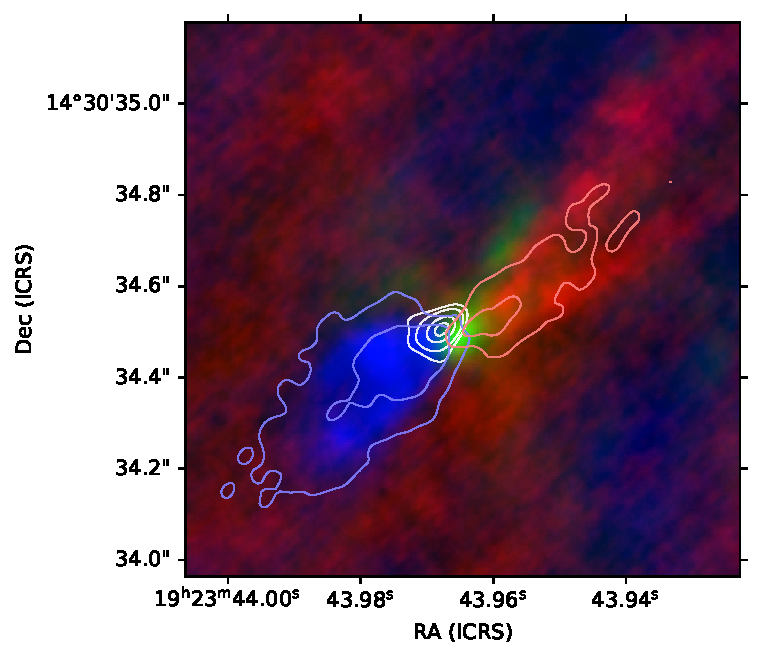
\includegraphics[width=\textwidth]{figures/W51e2e_sio_outflow_with_CS_contours.pdf}
    \caption{An image of the SiO 5-4 outflow (red and blue corresponding to
    red and blueshifted emission integrated over 74-118 \kms and -32 to 55
    \kms, respectively) with continuum shown in green.  The contours show
    integrated SiO J=2-1 over the same ranges in red (0.05, 0.1 K \kms) and
    blue (0.1, 0.2 K \kms), the CS 2-1
    maser in white (2000, 4000, 6000 peak intensity over -32 to 55 \kms),
    and the CS 1-0 maser in black (2000, 4000, 8000 K peak intensity over
    the range 55-74 \kms).  For both of the masers, the contours effectively
    indicate the beam size.}
    \label{fig:overlay}
\end{figure*}

The CS J=1-0 line is only seen as a single spatial component centered
at approximately $v_{lsr}=64 \pm 6$ \kms.  It is centered closer to the
central continuum source, but still slightly toward the blueshifted outflow.
The CS J=1-0 and J=2-1 masers are offset by $0.036\arcsec \pm 0.12$\arcsec
($190\pm60$ AU).

\begin{table*}[htp]
\centering
\caption{Line Fit Parameters}
\begin{tabular}{llllll}
    \label{tab:observations}
Line Name & Amplitude & $v_{LSR}$ & $\sigma_{FWHM}$ & RA (ICRS) & Dec (ICRS) \\
          &         K &      \kms &            \kms & $\deg$    & $\deg$ \\
\hline
CS J=1-0 &      6800 &$      65.5 \pm        0.7$ &$       7.3 \pm        1.2$ &$    290.9331902 \pm       0.0000025$ &$     14.5095795 \pm       0.0000021$ \\
CS J=2-1 &$      6700 \pm        200$ &$     34.50 \pm       0.07$ &$      5.27 \pm       0.17$ &$    290.9331982 \pm       0.0000025$ &$     14.5095852 \pm       0.0000021$ \\

\hline
\end{tabular}
\label{tab:linepars}
\par
Because of the coarse spectral resolution, the amplitude of the CS 1-0 line is
poorly constrained, and we report its fitted width and centroid assuming a
fixed amplitude of 6800 K.
\end{table*}


\begin{figure}[htp]
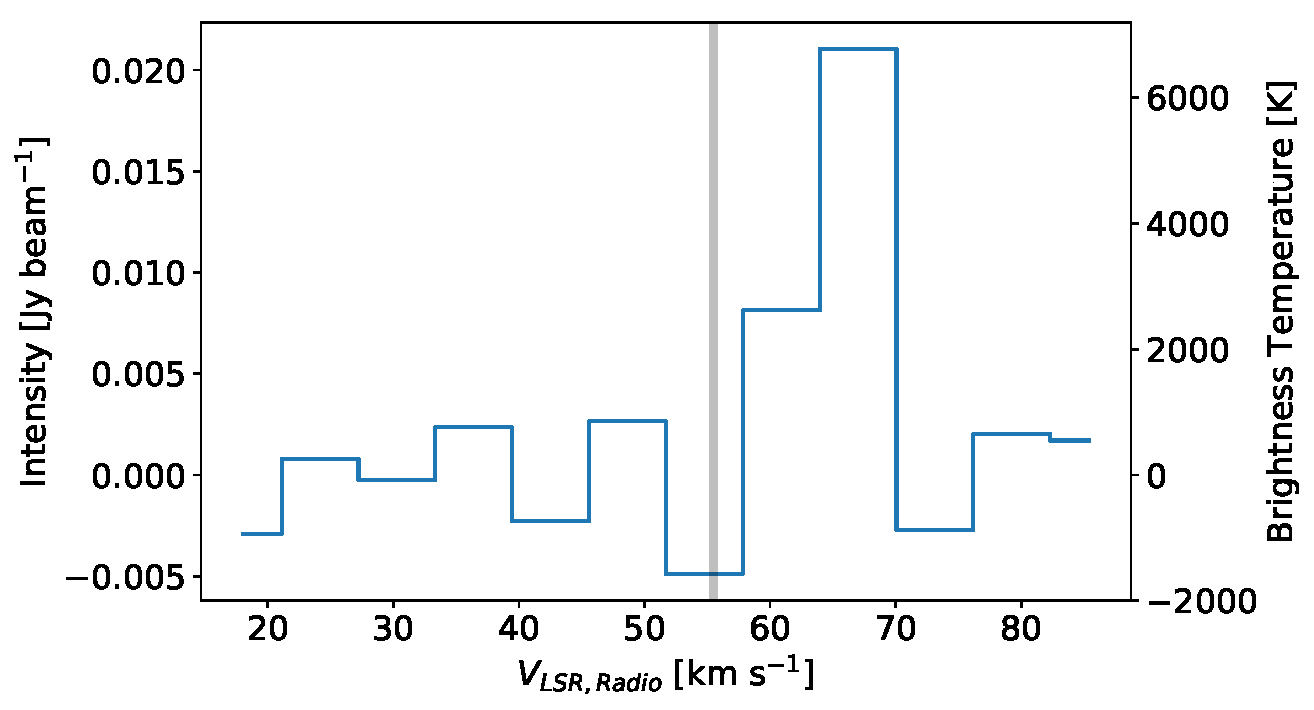
\includegraphics[width=0.45\textwidth]{figures/CS1-0_maser_JyandK.pdf}
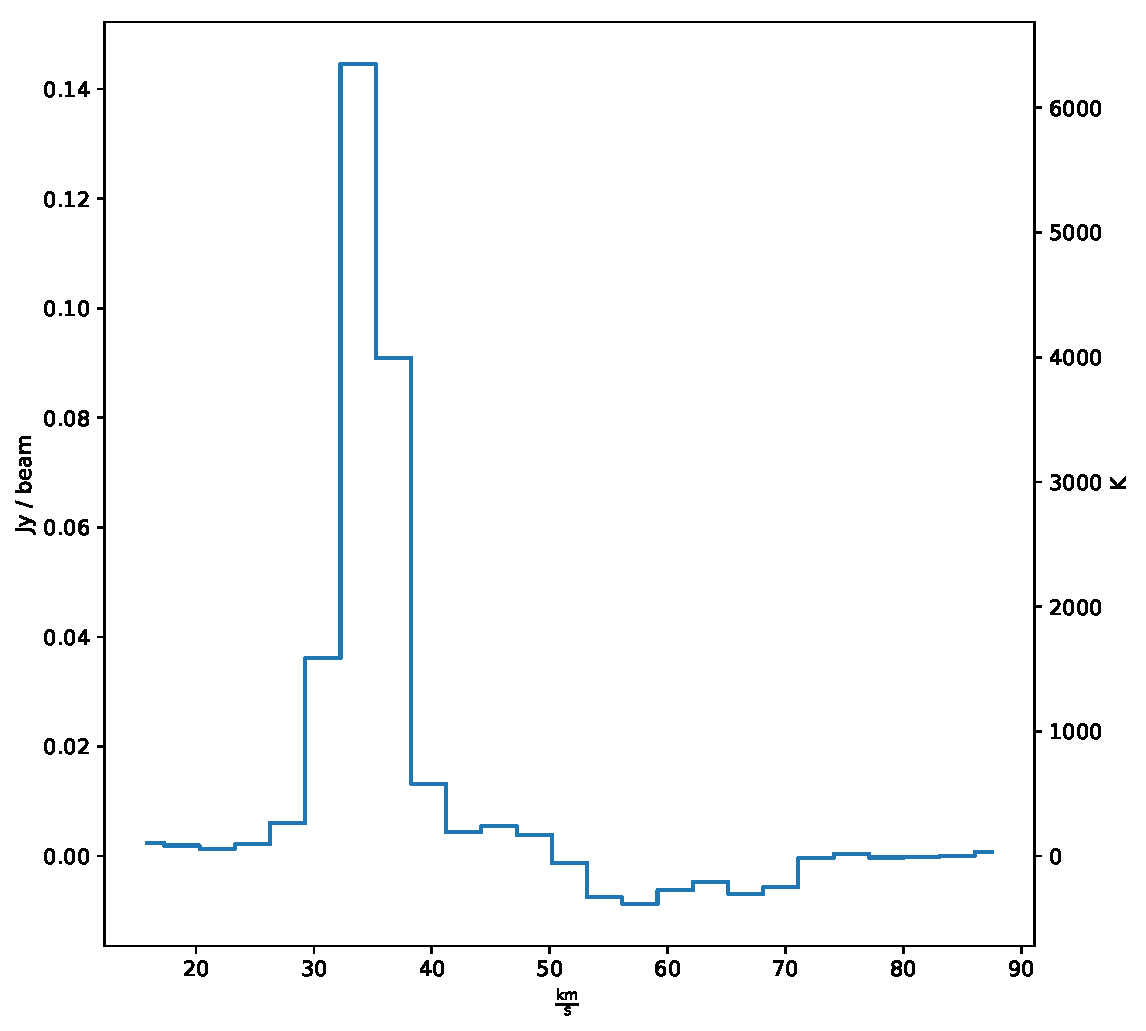
\includegraphics[width=0.45\textwidth]{figures/CS2-1_maser_JyandK.pdf}
\caption{Plots of the (a) CS J=1-0 and (b) CS J=2-1 spectra toward their
respective peak locations shown in Figure \ref{fig:overlay}.}
\label{fig:spectra}
\end{figure}


\section{Analysis}
The peak brightness of the observed lines is $\sim6800$ K at $\sim0.07\arcsec$
(350 AU at 3 mm) and $\sim0.04\arcsec$ (200 AU at 7 mm) resolution.  It is unlikely that the
molecules are in thermal equilibrium at $T_K \geq 6000$ K, since such high
temperatures would more likely result in dissociation of the molecules
\citep[e.g.,][]{Pattillo2018a}.
%TODO: check that it would actually dissociate

At the observed spectral resolution of 3 \kms, the CS J=2-1 line is marginally
resolved with FWHM=5.25 \kms ($\sigma=2.2 \kms$), and at 6 \kms resolution, the
CS J=1-0 line is unresolved.
The thermal line width of CS at 6000 K is FWHM=2.7 \kms ($\sigma=1.1$ \kms),
smaller than the measured width of CS J=2-1 and smaller than the resolution
of the CS J=1-0 data, so we cannot use these data to rule out a thermal
line width.
% The measured line width and the observed spectral resolution are both
% much greater than the thermal width for CS at 6000 K, $v_{therm}\approx1~\kms$.
%we cannot conclude anything about the intrinsic line width.

While both transitions have a consistent peak brightness of $\sim6800$ K,
which is below that typical of maser transitions in other molecules, these
emission peaks are at different velocities and may be from different spatial
locations (separated
by about 190 AU), and therefore they are not emitted by the same material.
This velocity difference rules out a thermal origin for either transition,
since thermal lines should have comparable brightness in both transitions
at similar velocities.

The separation between the two maser spots in position and velocity hints
that the masers could be produced at the extreme ends of a disk orbiting
a central protostar.  The coincidence between the CS 1-0 maser peak and
the 1 mm continuum peak is evidence against this hypothesis, but is not definitive:
the midpoint of the SiO outflow is also not coincident with the 1 mm continuum
peak.

If we assume the masers trace orbiting material, their velocity and spatial
separation can be used to infer the central source mass.  At a separation of 30
\kms and 190 AU, assuming the masers come from opposite ends of a disk such
that $v_{orb}=15\pm1$~\kms and $R_{disk}=95\pm30$~AU, the implied contained mass is
$M=24_{-10}^{+12}$~\msun.  This mass is of order that suggested by
\citet{Ginsburg2017a} and \citet{Goddi2018a} based on luminosity estimates.
However, the velocity separation also hints that these masers may be produced
in the outflow rather than in a disk.  In that case, the orbital analysis
is not valid.


Our data also include the W51 IRS2/north and W51e8 HMYSOs
\citep{Ginsburg2017a}.  No compact and bright CS emission sources were detected
toward either of these HMYSO candidates, with a peak CS 2-1 flux limit ${S_{98
\mathrm{GHz}} \leq 15 \mathrm{mJy~\perbeam}}$, an order of magnitude fainter
than the peaks seen in W51e2e.  However, plentiful extended CS 2-1 emission is
seen around each of the HMYSOs.  This difference indicates that there is
something unique about the chemistry, geometry, or excitation in the W51e2e
that drives these particular maser transitions.

The detection of CS 1-0 emission at $\sim65$ \kms is actually quite surprising,
since W51e2e is deeply embedded in a high column density molecular medium that
covers this velocity.  Since the maser is detected, there must either be a hole
through which we are seeing the compact emission, or the foreground cloud's CS
is highly excited and has a minimal ground-state population at 65 \kms; the
latter explanation is more likely.  The J=2-1 transition at 34.5 \kms is not
subject to this concern, since there is no foreground material at that
velocity, but it is possible that a 2-1 maser exists near 65 \kms and is fully
absorbed by foreground cloud material.

%It is possible that a region within a few AU of the the central MYSO is heated
%to such high temperatures.  To provide a high enough column density of CS
%to exhibit the observed brightness, this region may have developed an
%equilibrium between CS formation and destruction.

\begin{figure*}
    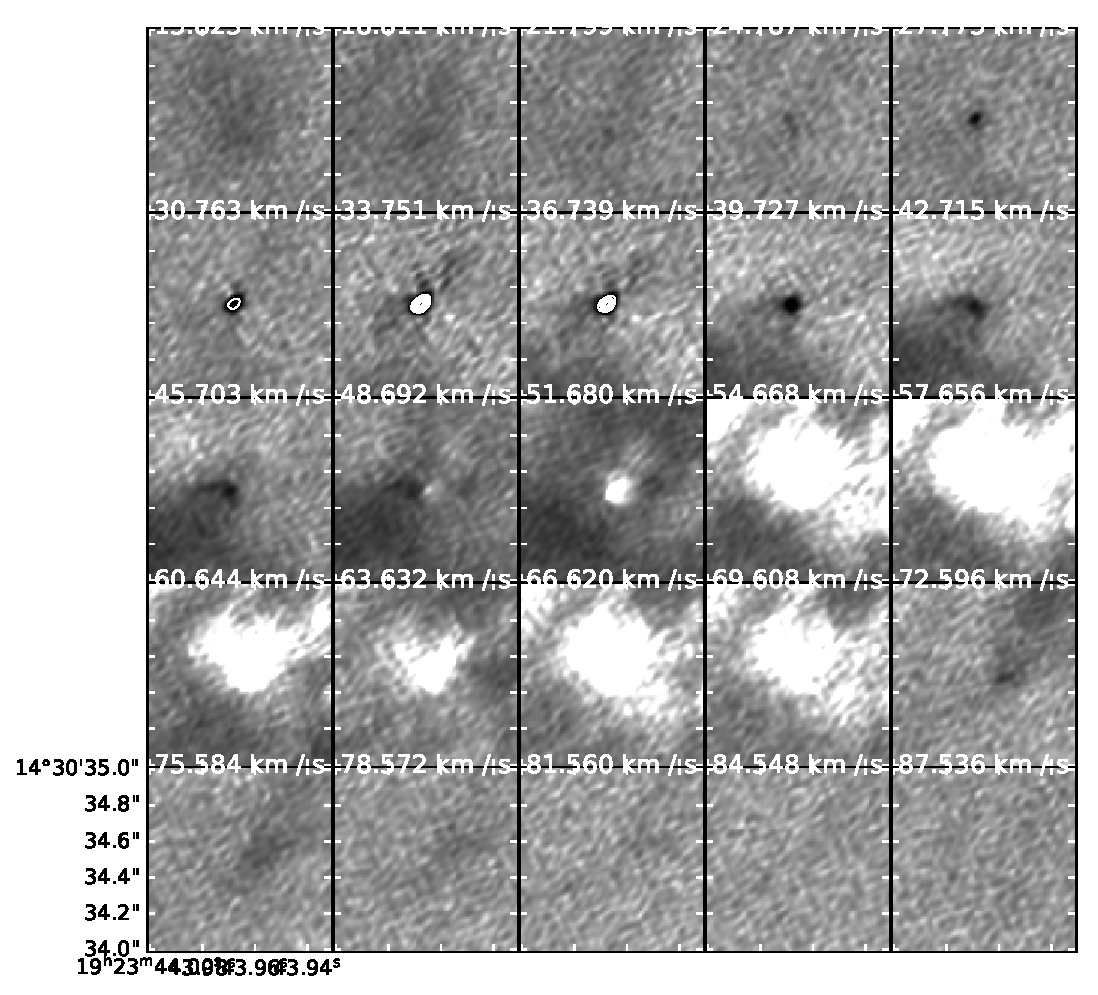
\includegraphics[]{figures/CS_maser_channel_maps.pdf}
    \caption{Channel maps of the CS J=2-1 transition.  Channels are 3 \kms
    wide.  Darker colors indicate higher intensity.  Contours are overlaid at
    [0.02,0.04,0.06,0.08,0.1,0.125] Jy/beam.  Absorption against the continuum
    is evident in white from 50-70 \kms.  The redshifted outflow is faint but still
    detected at
    $\sim72.5\kms$.
    }
    \label{fig:channelmaps}
\end{figure*}

\section{Conclusions}
We have detected two emission lines from the J=2-1 and J=1-0 transitions of CS
with high brightness temperature indicating that these lines are masers.
This is the first reported detection of maser emission from CS.
While the HMYSO W51e2e exhibits these masers, several neighboring HMYSOs that
are similar in luminosity, core mass, and apparent evolutionary stage
do not.  The presence of two CS masers from different rotational states
at different velocities and locations in the source suggest that there is something
unique about this object's radiation field, geometry, or chemistry that
promotes CS maser formation.

These CS masers join a growing list of rarely-detected maser transitions
that may trace a unique phase in the formation of high-mass protostars.
Like the NH$_3$, H$_2$CO, and SiO masers, there are only 1-10 known sources of
each of these masers.  Curiously, W51 North, a known host of NH$_3$ and SiO masers,
does not exhibit any CS maser emission.  Other HMYSOs should be searched for
masers in these transitions to determine how common they are.

\textbf{Acknowledgements}
We thank Todd Hunter for providing literature references on CS masers and
Lorant Sjouwerman for discussion about a lack of CS masers in AGB stars.

\textbf{Software}
This paper used \texttt{astropy}
\citep{Astropy-Collaboration2013a,Astropy-Collaboration2018a},
\texttt{pyspeckit} \citep{Ginsburg2011c}, and CASA \citep{McMullin2007a}.

\appendix
\section{Velocity check}
We carefully checked the velocity measurements in the VLA data, since an offset
of a few channels is comparable to the Earth's motion and we are using a
continuum band to infer velocity information.  The observations we analyze were
taken on December 26 and 30, 2016 and January 7, 2017.  On these dates, the
topocentric-to-barycentric velocity corrections are -9.0, -7.4, and -4.1 \kms,
respectively.  The barycentric-to-LSR correction toward W51 is 16.5 \kms.  The
observed CS J=1-0 peak is in channel 24 (zero-indexed) of spectral window 26,
which has channel 0 at  48957.667, 48957.932, and 48958.478 MHz, respectively,
for each of the three observations.  The channel width is 1 MHz.  The LSR
velocity of the CS J=1-0 peak intensity channel is at 64.3 \kms on all three
dates.  This value is consistent with our reported velocity of
$v_{LSR}(\mathrm{CS~J=}1-0) = 65.5 \pm 0.7 \kms$.

No such sanity check is needed for the ALMA data, since the channel maps
clearly show the outflow at appropriate velocities with morphology that matches
the SiO outflow seen at both 1 mm and 3 mm.

\section{Variability check}
We also checked for variability in the CS 1-0 maser, and found no evidence for
variability across four observing epochs (2016-10-02, 2016-12-26, 2016-12-30,
2017-01-07; the former was not included in our merged data set because we were unable
to perform bandpass calibration).  The position remained constant and the flux
remained consistent to within single-epoch observing errors.

\bibliographystyle{aasjournal}
\bibliography{extracted}
\end{document}
